\documentclass[12pt]{article}  % 官方要求字号不小于 12 号,此处选择 12 号字体

% 本模板不需要填写年份,以当前电脑时间自动生成
% 请在以下的方括号中填写队伍控制号
\usepackage[UTF8]{ctex}
\usepackage{float}
\usepackage[2510625]{easymcm}  % 载入 EasyMCM 模板文件
\problem{B}  % 请在此处填写题号
% \usepackage{mathptmx}  % 这是 Times 字体,中规中矩 
\usepackage{mathpazo}  % 这是 COMAP 官方杂志采用的更好看的 Palatino 字体,可替代以上的 mathptmx 宏包

\title{An MCM Paper Made by Team 2510625}  % 标题

% 如需要修改题头(默认为 MCM/ICM),请使用以下命令(此处修改为 MCM)
%\renewcommand{\contest}{MCM}

% 文档开始
\begin{document}

% 此处填写摘要内容
\begin{abstract}
    Here is the abstract of your paper.

    对于第一个模型,游客是唯一的决策变量,同时为了达到最大化环境质量和社会满意度的需求,模型采取了\textbf{多目标建模的方法},最后使用\textbf{帕累托最优法}来确定多组最优解并为决策提供相应的结果建议。在这个模型中,社会满意度由两个部分组成,一是当地居民的满意度,二是游客的满意度,并分别取0.5的权重相加作为最终的社会满意度。人数主要由两个因素来进行限制,一是当地水资源的限制,而是当地废物处理的能力的限制。环境的质量由三个因素来考虑,水资源的消耗量,CO_2的排放量以及废物的增加量。

    Secondly, that is ...

    Finally, that is ...

    % 美赛论文中无需注明关键字。若您一定要使用,
    % 请将以下两行的注释号 '%' 去除,以使其生效
    % \vspace{5pt}
    % \textbf{Keywords}: MATLAB, mathematics, LaTeX.

\end{abstract}

\maketitle  % 生成 Summary Sheet
\tableofcontents  % 生成目录


% 正文开始
\section{Introduction}
\subsection{Problem Background}
Here is the problem background. Three major problems are discussed in this paper, which are:
\begin{itemize}
    \item \textbf{地理位置:}朱诺市是美国阿拉斯加州的首府,位于阿拉斯加东南部,拥有约30,000名居民。这座城市以其丰富的自然资源、独特的地理位置和迷人的自然景观而闻名,是许多游客前往阿拉斯加的首选目的地之一。朱诺市不仅是阿拉斯加的政治中心,也是一个重要的旅游枢纽,以其冰川、雨林和丰富的野生动物资源吸引着来自世界各地的游客。
    \item \textbf{旅游现状:}近年来,朱诺市的旅游业经历了迅猛的发展,尤其是在邮轮旅游方面。2023年,朱诺市创下了接待160万邮轮游客的纪录,单日最多接待7艘大型邮轮,游客数量高达20,000人。\cite{1}这些游客为城市带来了可观的经济收益,约3.75亿美元。\cite{2}然而,这种快速发展的旅游业也带来了一系列问题,尤其是与过度旅游相关的挑战。
    \item \textbf{环境影响:}朱诺市的门登霍尔冰川是该市的主要旅游景点之一,但近年来由于气温上升,冰川正在快速消退。自2007年以来,冰川已经后退了相当于八个足球场的距离。这种环境变化不仅对自然景观造成了破坏,也引发了当地居民对旅游业可持续性的担忧。\cite{3}
\end{itemize}

\begin{figure}[H]
\centering
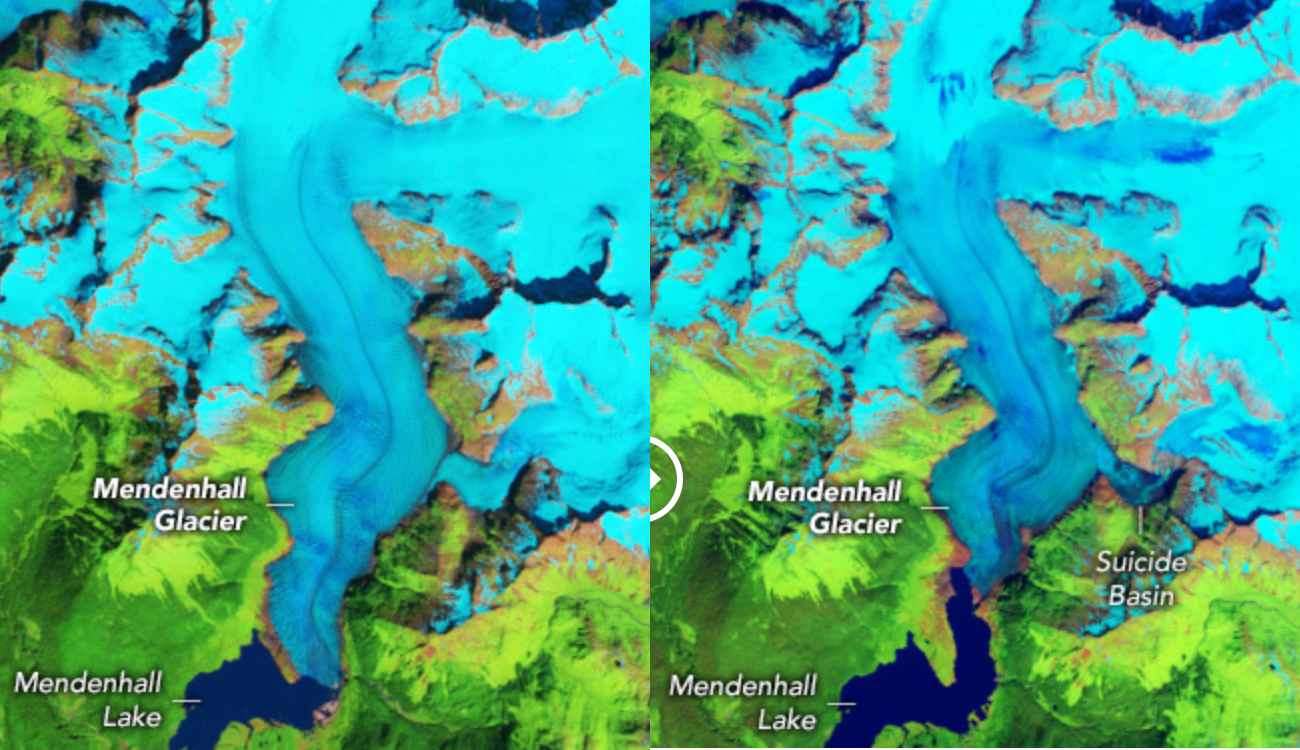
\includegraphics[width=.8\textwidth]{glacier.png}
\caption{glacier}\label{fig:glacier}
\end{figure}

\subsection{Problem Restatement and Analysis}
\begin{itemize}
    \item \textbf{Problem1: }建立一个可持续旅游产业的模型,它应当满足最大化收入,最大化环境质量且最大化社会满意度并对其进行敏感性分析。
    \item \textbf{Problem2: }建立一个模型去解决游客分流到其他人流量比较小的景点,这也是增加收入减少区域压力的措施。
    \item \textbf{Problem3: }展示模型如何可以适应另一个受过度旅游影响的旅游目的地,应当去获取另一个城市的相关信息并用模型进行预测。
    \item \textbf{Problem4: }展示模型随着具体措施会发生的变化以此来为决策者提供更好的建议,比如加酒店税、游客费用、每日游客数量上限以及限制酒精销售和消费等。
    \item \textbf{An article: }为朱诺市旅游局写一封一页的备忘录,概述结果的预测、各种措施的影响以及对如何优化结果的建议。
\end{itemize}

\subsection{Our work}
\begin{enumerate}[\bfseries 1)]
    \item 
    \item We do ...
    \item We do ...
\end{enumerate}

\section{Preparation of the Models}
\subsection{Assumptions}

\subsection{Notations}
The primary notations used in this paper are listed in Table \ref{tb:notation}.

% 三线表示例
\begin{table}[H]
\begin{center}
\caption{Notations}
\begin{tabular}{>{\centering\arraybackslash}m{4cm} >{\centering\arraybackslash}m{10cm}}
	\toprule
	Symbol & Definition\\
	\midrule
	$N_t$ & Number of tourists\\
    $N_{tmax}$ & Maximum number of tourists allowed per day\\
	$\tau _t$ & Tourists taxes or surcharges per tourist\\
	$P_t$ & Average spending per tourists\\
    $P_b$ & Infrastructuren investiment expenditure\\
    $P_e$ & Environment protection investiment expenditure\\
    $CO_{2p}$ & Carbon emissions per person\\
    $R_e$ & Total revenue\\
    $C_h$ & Hidden cost\\
    $E$ & Environment Quality Index\\
    $R_{nature}$ & Nature Recovery\\
    $S_{residents}$ & Residents' satisfaction\\
    $S_{tourists}$ & Tourists' satisfaction\\
    $S$ & Societal satisfaction\\
    $C_{infra}$ & Infractructure carrying capacity\\
	\bottomrule
\end{tabular}\label{tb:notation}
\end{center}
\end{table}

\section{The Models}
\subsection{Model 1}
\subsubsection{Details about Model 1}

\begin{equation}
	R_{e}(N_{t},P_{t}) = P_{t}N_{t}
	\end{equation}
	\begin{equation}
	E=k_{1}(CO_{2p}N_{t}-C_{base})+k_{2}\frac{N_{t}}{C_{waste}}+k_{3}\frac{N_{t}}{C_{water}}
	\end{equation}
	\begin{equation}
	\begin{cases}
		S_{residents}=a_{1}N_{t}^2+a_{2}N_{t} + b_{1} \\
		S=k_{4}S_{residents}
	\end{cases}
	\end{equation}
	\begin{equation}
	\begin{cases}
		\frac{\mathrm{d}C_{waste}}{\mathrm{d}t}=\alpha_1P_{waste} \\
		\frac{\mathrm{d}C_{water}}{\mathrm{d}t}=\alpha_2P_{water} \\
		\frac{\mathrm{d}C_{base}}{\mathrm{d}t}=\alpha_3P_e \\
	\end{cases}
	\end{equation}
	\begin{equation}
	\begin{cases}
	P_{waste} = k_5\tau_tR_e\\
	P_{water} = k_6\tau_tR_e\\
	P_{e}=k_7\tau_{t}R_e \\
	k_5+k_6+k_7 \leqslant 0.4
	\end{cases}
	\end{equation}
	\begin{equation}
		Target equation:Z=R_e+S-E
	\end{equation}

\subsection{Model 2}
\subsubsection{Conclusion of Model 2}
The results are shown in Figure \ref{fig:result}, where $t$ denotes the time in seconds, and $c$ refers to the concentration of water in the boiler.

\begin{figure}[htbp]
\centering
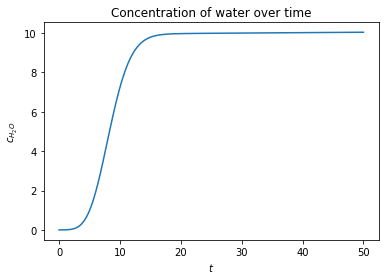
\includegraphics[width=.8\textwidth]{water.png}
\caption{The result of Model 2}\label{fig:result}
\end{figure}

\clearpage
\subsubsection{Commetary on Model 2}
The instance of long and wide tables are shown in Table \ref{tb:longtable}.

% 长表格示例,更多用法请参考 longtable 宏包文档
% 以下环境及对应参数可实现表格内的自动换行与表格的自动断页
% 您也可以选择自行载入 tabularx 宏包,并通过 X 参数指定对应列自动换行
\begin{longtable}{ p{4em} p{14em} p{14em} }
\caption{Basic Information about Three Main Continents (scratched from Wikipedia)}
\label{tb:longtable}\\
\toprule
Continent & Description & Information \\
\midrule
Africa & Africa Continent is surrounded by the Mediterranean Sea to the
north, the Isthmus of Suez and the Red Sea to the northeast, the Indian
Ocean to the southeast and the Atlantic Ocean to the west. &
At about 30.3 million km$^2$ including adjacent islands, it covers 6\%
of Earth's total surface area and 20\% of its land area. With 1.3
billion people as of 2018, it accounts for about 16\% of the world's
human population. \\
\midrule
Asia & Asia is Earth's largest and most populous continent which
located primarily in the Eastern and Northern Hemispheres.
It shares the continental landmass of Eurasia with the continent
of Europe and the continental landmass of Afro-Eurasia with both
Europe and Africa. &
Asia covers an area of 44,579,000 square kilometres, about 30\%
of Earth's total land area and 8.7\% of the Earth's total surface
area. Its 4.5 billion people (as of June 2019) constitute roughly
60\% of the world's population. \\
\midrule
Europe & Europe is a continent located entirely in the Northern
Hemisphere and mostly in the Eastern Hemisphere. It comprises the
westernmost part of Eurasia and is bordered by the Arctic Ocean to
the north, the Atlantic Ocean to the west, the Mediterranean Sea to
the south, and Asia to the east. &
Europe covers about 10,180,000 km$^2$, or 2\% of the Earth's surface
(6.8\% of land area), making it the second smallest
continent. Europe had a total population of about 741 million (about
11\% of the world population) as of 2018. \\
\bottomrule
\end{longtable}

Figure \ref{fig:subfigures} gives an example of subfigures. Figure \ref{subfig:left} is on the left, and Figure \ref{subfig:right} is on the right.

% 子图(多图并列)示例,更多用法请参考 subfigure 宏包文档
% 如果您只希望几张图并列,不需要额外的 caption,那么在 figure 环境中
% 连续插入总宽度不超过 \textwidth 的多个 \includegraphics 命令即可
\begin{figure}[htbp]
\centering
\begin{subfigure}[b]{.4\textwidth}
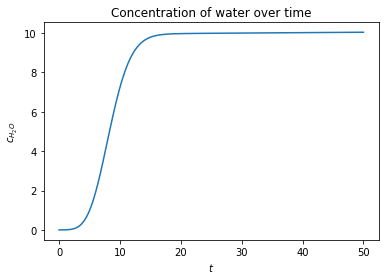
\includegraphics[width=\textwidth]{water.png}
\caption{Image on the left}\label{subfig:left}
\end{subfigure}
\begin{subfigure}[b]{.4\textwidth}
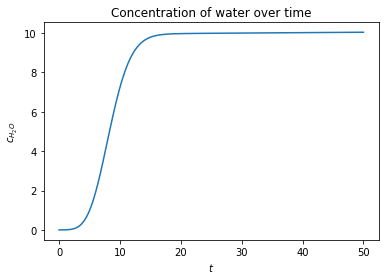
\includegraphics[width=\textwidth]{water.png}
\caption{Image on the right}\label{subfig:right}
\end{subfigure}
\caption{Two images}\label{fig:subfigures}
\end{figure}

\section{Strengths and Weaknesses}
\subsection{Strengths}
\begin{itemize}
    \item First one...
    \item Second one ...
\end{itemize}

\subsection{Weaknesses}
\begin{itemize}
    \item Only one ...
 \end{itemize}


% 以下为信件/备忘录部分,不需要可自行去掉
% 如有需要可将整个 letter 环境移动到文章开头或中间
% 请在第二个花括号内填写标题,如「信件」(Letter)或「备忘录」(Memorandum)
\begin{letter}{Memorandum}
\begin{flushleft}  % 左对齐环境,无首行缩进
\textbf{To:} Heishan Yan\\
\textbf{From:} Team 1234567\\
\textbf{Date:} October 1st, 2019\\
\textbf{Subject:} A better choice than MS Word: \LaTeX
\end{flushleft}

In the memo, we want to introduce you an alternate typesetting program to the prevailing MS Word: \textbf{\LaTeX}. In fact, the history of \LaTeX\ is even longer than that of MS Word. In 1970s, the famous computer scientist Donald Knuth first came out with a typesetting program, which named \TeX\ \ldots

Firstly, \ldots

Secondly, \ldots

Lastly, \ldots

According to all those mentioned above, it is really worth to have a try on \LaTeX! 
\end{letter}


% 参考文献,此处以 MLA 引用格式为例

\begin{thebibliography}{99}
\bibitem{1} \url{https://abc7.com/post/juneau-alaska-cruise-ship-limits-overtourism/15048713/}
\bibitem{2} \url{https://juneau.org/wp-content/uploads/2024/01/CBJ-Cruise-Impacts-2023-Report-1.22.24.pdf}
\bibitem{3} \url{https://alaskapublic.org/2023/08/07/crammed-with-tourists-juneau-wonders-what-will-happen-as-mendenhall-glacier-recedes/}
\bibitem{4} \emph{A simple, easy \LaTeX\ template for MCM/ICM: EasyMCM}. (2018). Retrieved December 1, 2019, from\url{https://www.cnblogs.com/xjtu-blacksmith/p/easymcm.html}
\end{thebibliography}


% 以下为附录内容
% 如您的论文中不需要附录,请自行删除
\begin{subappendices}  % 附录环境

\section{Appendix A: Further on \LaTeX}
To clarify the importance of using \LaTeX\ in MCM or ICM, several points need to be covered, which are \ldots

To be more specific, \ldots

All in all, \ldots

Anyway, nobody \textbf{really} needs such appendix \ldots

\section{Appendix B: Program Codes}
Here are the program codes we used in our research.

% 代码环境示例三则
% 如您的论文不需要展示代码,请删除
% 更多用法,请参考 listings 宏包文档

% Python 代码示例
\begin{lstlisting}[language=Python, name={test.py}]
# Python code example
for i in range(10):
    print('Hello, world!')
\end{lstlisting}

% MATLAB 代码示例
\begin{lstlisting}[language=MATLAB, name={test.m}]
% MATLAB code example
for i = 1:10
    disp("hello, world!");
end
\end{lstlisting}

% C++ 代码示例
\begin{lstlisting}[language=C++, name={test.cpp}]
// C++ code example
#include <iostream>
using namespace std;

int main() {
    for (int i = 0; i < 10; i++)
        cout << "hello, world" << endl;
    return 0;
}
\end{lstlisting}

\end{subappendices}  % 附录内容结束

\end{document}  % 结束
